% ==============================================================================
% ================================= Aufgabe 5 =================================
% ==============================================================================

\chapter{Aufgabe 5: Speichern der Umfragedaten}
\label{chap:aufgabe5}
\thispagestyle{fancy}

In dieser Aufgabe wird die Datei \texttt{save.php} implementiert, die die Umfragedaten aus dem POST-Request entgegennimmt und in der Datenbank speichert.

\section{Logik der \texttt{save.php}}

Die Datei \texttt{save.php} übernimmt folgende Aufgaben:

\begin{enumerate}
    \item Entgegennahme der POST-Daten aus dem Formular der \texttt{survey.php}.
    \item Validierung der empfangenen Daten (\textit{insbesondere der \texttt{UserId}}).
    \item Erzeugung des aktuellen Datums mit \texttt{date(\textit{'Y-m-d'})}.
    \item Speicherung der Daten in der Tabelle \texttt{survey\_table}.
    \item Anzeige einer Erfolgsmeldung mit Link zum Report.
\end{enumerate}

\subsection{Vollständiger Quellcode}

\lstinputlisting[
    language=php,
    caption={Speicherung der Umfragedaten in \texttt{save.php}},
    label={lst:save-php}
]{asset/code/Aufgabe5.tex}

\subsection{Erläuterung der einzelnen Bestandteile}

\subsubsection{Auslesen der POST-Daten}

Die POST-Daten werden wie folgt ausgelesen:

\begin{lstlisting}[language=php]
$userId = isset($_POST['userId']) ? (int)$_POST['userId'] : 0;
$q1     = isset($_POST['Q1']) ? trim($_POST['Q1']) : '';
\end{lstlisting}

\subsubsection{Datumserzeugung}

Das aktuelle Datum wird im Format \texttt{YYYY-MM-DD} erzeugt:

\begin{lstlisting}[language=php]
$datum = date('Y-m-d');
\end{lstlisting}

\subsubsection{Prepared Statement für INSERT}

Zur Vermeidung von \acs{SQL}-Injection wird ein Prepared Statement verwendet:

\begin{lstlisting}[language=php]
$stmt = $pdo->prepare("
    INSERT INTO survey_table (UserId, Datum, Q1, Q2, Q3, Q4, Q5)
    VALUES (?, ?, ?, ?, ?, ?, ?)
");
$stmt->execute([$userId, $datum, $q1, $q2, $q3, $q4, $q5]);
\end{lstlisting}

\subsection{Erfolgsmeldung}

Nach erfolgreicher Speicherung wird folgende Meldung angezeigt:

\begin{figure}[h]
    \centering
    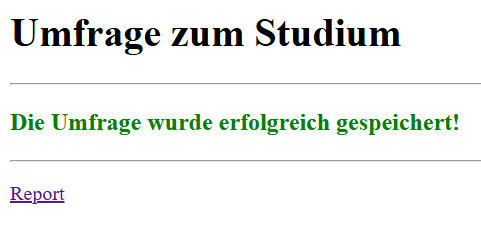
\includegraphics[width=0.6\textwidth]{./asset/image/Aufgabe5.png}
    \caption[Erfolgsmeldung nach dem Speichern (\textit{Quelle: Eigene Darstellung})]
            {Erfolgsmeldung nach dem Speichern (\textit{Quelle: Eigene Darstellung})\\ 
            \url{http://localhost/survey/save.php}}
    \label{fig:save_success}
\end{figure}

\section{Datenbankstruktur der \texttt{survey\_table}}

Die Tabelle \texttt{survey\_table} wurde in Aufgabe 1 mit folgender Struktur angelegt:

\begin{table}[h]
\centering
\begin{tabular}{|l|l|l|}
\hline
\textbf{Spalte} & \textbf{Datentyp} & \textbf{Besonderheit} \\
\hline
Id & INT & Primary Key, Auto Increment \\
UserId & INT & NOT NULL, Fremdschlüssel \\
Datum & DATE & NOT NULL \\
Q1 & VARCHAR(255) & NOT NULL \\
Q2 & VARCHAR(255) & NOT NULL \\
Q3 & VARCHAR(255) & NOT NULL \\
Q4 & VARCHAR(255) & NOT NULL \\
Q5 & VARCHAR(255) & NOT NULL \\
\hline
\end{tabular}
\caption{Struktur der Tabelle \texttt{survey\_table}}
\label{tab:survey_table}
\end{table}

Die Spalte \texttt{Datum} speichert das Datum der Umfrageteilnahme im Format \texttt{YYYY-MM-DD}.

\section{Zusammenfassung}

Die Speicherung der Umfragedaten wurde erfolgreich implementiert:

\begin{itemize}
    \item Die POST-Daten werden aus dem Formular ausgelesen.
    \item Das aktuelle Datum wird mit \texttt{date()} erzeugt.
    \item Die Daten werden in \texttt{survey\_table} gespeichert.
    \item Bei Erfolg wird eine Meldung mit Link zum Report angezeigt.
    \item Bei Fehlern wird eine entsprechende Fehlermeldung ausgegeben.
\end{itemize}

Die Datei \texttt{save.php} liegt unter folgendem Pfad:

\begin{forest}
    for tree={
        font=\ttfamily,
        grow'=0,
        child anchor=west,
        parent anchor=south,
        anchor=west,
        calign=first,
        edge path={
            \noexpand\path [draw, \forestoption{edge}] (!u.south west) +(10pt,0) |- node[fill,inner sep=1.5pt] {} (.child anchor)\forestoption{edge label};
        },
        before typesetting nodes={
            if n=1{
                insert before={[,phantom,calign with current]}
            }{}
        },
        fit=band,
        before computing xy={l=22pt},
    }
    [\textbf{C:\textbackslash xampp\textbackslash htdocs\textbackslash survey}
        [\textbf{save.php}]
    ]
\end{forest}

Die Anwendung ist nun bereit für die Auswertung der Umfragedaten.

% ==============================================================================
% =================================== Aufgabe 5 ================================
% ==============================================================================